\chapter{Implementation Details}
\label{chap:Implementation Details}
We find the low-level implementation of the data structures and algorithms mentioned so far is an important part of acheiving performance. Recent work by Sidlauskas \ea~\cite{Sidlauskas2014-ef} claims that based on empirical performance findings, there is a challenge about concluding about data structures and algorithms, and that this is more important in an in-memory setting.

It is all about reducing the number of branches, operate on multiple values at a time, cache awareness, and avoid extra layers of indirection.
\newpage

\section{Background information on modern CPUs}
\label{sec:Background information on modern CPUs}
Modern CPUs has pipelining with dependencies, branch predictions. In addition, 30\% of the instructions are loads and stores \cite{Boncz2005-wj}. \textbf{All in all, CPUs have become highly complex devices where instruction throughput of a processor can vary by orders of magnitude}. \todo{More stuff here in Boncz2005-wj}

\section{Branch avoidance}
\label{sec:Branch avoidance}
\ffigure{img/branch-selectivity.png}{Courtesy of \cite{Boncz2005-wj}.}{fig:branch-selectivity}
Avoiding branches in when processing queries is an important factor for performance. Modern CPUs have branch predictors, but if a branch is mispredicted, the whole pipeline must be flushed. If branches are taken with a probability of 50\%, branch prediction is very expensive \cite{Neumann2011-uq}. This can happen in processing a query with 50\% selectivity. See Figure \ref{fig:branch-selectivity}.

A common way of avoiding branches, is to leave out short circuiting from the code. Short circuiting is the technique where you only evaluate one predicate at a time, or one tuple at a time, and only proceed if the predicate is true or the tuple is valid from the candidate. This results in many if statements within the query. Short circuiting will only improve performance on low selectivity queries \cite{Johnson2008-cp}.

\blink~\cite{Johnson2008-cp} does not short circuit between tuples, only between blocks. Hence, if a block is selected for scanning, all tuplets are evaluated and the result is a candidate vector.

Branch avoidance is also imortant when decompressing. In the compression algorithm presented by Zukowski \ea~\cite{Zukowski2006-oz}, careful implementation avoids if-then-else in inner loops.

\subsection{Loop pipelining}
\label{sub:Loop pipelining}
The absence of loop pipelining can have dramatic effects on query performance. Boncz \ea~\cite{Boncz2005-wj} show how the \mysql uses 49 cycles per tuple due to the absence of loop pipelining.

In order to ensure proper loop pipeline behavior, compilers must know that pointers do not overlap, such that loop unrolling can be used. CPU primitives expose to the compiler that processing a tuple is independent from the others. This is also important in the decompression and compression step \cite{Zukowski2006-oz}

A simple technique is presented by Zukowski \ea~\cite{Zukowski2006-oz} is the \term{Two pointer solution}, where you use two pointers in a loop instead of one, and cut the number of iterations in half.

\subsection{Macro expansions}
\label{sub:Macro expansions}
To avoid branches and exploin loop pipelining, two techniques are used. The first one is to use macro expansions when developing the database. \monetdb~\cite{Boncz2002-yj} uses macro expansions such that multiple functions per operator are compiled for different data types. All

\subsection{Compiling into machine code}
\label{sub:Compiling into machine code}
\begin{figure}
  \centering
  \begin{subfigure}{0.45\textwidth}
    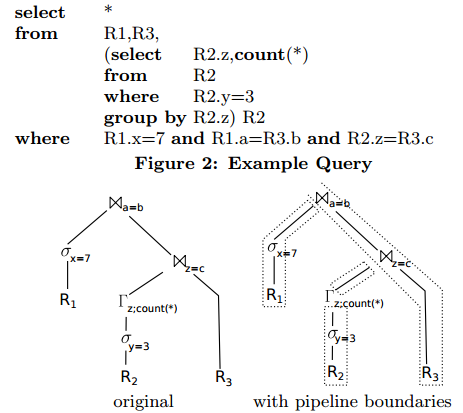
\includegraphics[width=\textwidth]{img/pipeline-boundary-1.png}
    \caption{...}
    \label{fig:pipeline-boundary-1} 
  \end{subfigure}
  \begin{subfigure}{0.45\textwidth}
    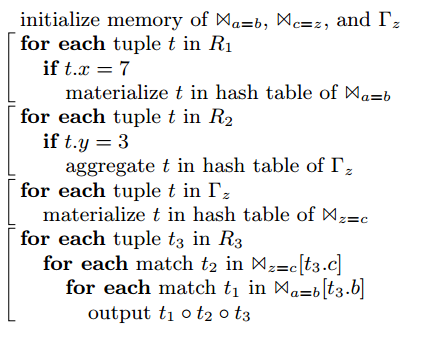
\includegraphics[width=\textwidth]{img/pipeline-boundary-2.png}
    \caption{...}
    \label{fig:pipeline-boundary-2} 
  \end{subfigure}
  \caption{Pipeline boundaries. Courtesy of \cite{Neumann2011-uq}.}
  \label{fig:pipeline-boundary} 
\end{figure}
The work by Neumann \ea~\cite{Neumann2011-uq} explains how queries are compiled into native machine code using the LLVM compiller framework. Doing this, the processing of queries are data centric and not operator centric. Classical query processing always wipes the CPU registers, but in their solution they push tuple values until a pipeline is broken. They tried using the C++ compiler, but it turned out too slow. Therefore, the major application was developed in C++. According to the developers behind the \hyper~database, compilation of queries will increase the performance of ad-hoc queries because ...

The technique of compiling queries and data structures are used by several databases. \blink~\cite{Barber2012-xt}, \ibm~\cite{Raman2013-em}, \vertica~\cite{Lamb2012-kg} generates a different code per frequency partition, since the dictionaries are different. 


In terms of application specific compliation, it is not only a question of precompiling the queries, but also compiling the column stores and other data structures directly. \mssql~\cite{Delaney2014-ip} memory database are natively compiled into DLLs and queries and stored procedures are run as native code.\qlikview~\cite{noauthor_undated-js} data is compiled straight into machine code, and temporary toolkup tables are used. They claim a performance increase of 10\%.

\section{Cache awareness}
\label{sec:Cache awareness}
In addition to avoiding branches and optimizing for loop pipelining, the implementation must also be aware of the computer cache. The CPU caches are important, since 30\% of the instructions given to the CPU are loads and stores \cite{Boncz2005-wj}. There are multiple ways to go about cache awareness. The developers behind \exasol claims that high level of data locality is one of the key factors for performance \cite{Exasol2014-xh}.

Perhaps the most important, is that algorithms must be cache aware \cite{Farber2012-vh}. In terms of database algorithm, several cache aware variants have been proposed. \monetdb~\cite{Boncz2002-yj} introduce a clever clustering algorithm called \term{radix cluster}, where cache utilization is maximized by performing muliple passes over the data. \oracle~\cite{Lahiri2015-mz} uses an algorithm known as \term{Vector Group By}, which is a compact multidimensional array for storing aggregate results.

Not only is data locality important, but also code locality \cite{Neumann2011-uq}. When compiling queries into code, there is a question of code size versus function definitions. If no functions are generated, there is an exponetial growth of code. Therefore, a balance must be found, but the important thing is that a hot path never cross a function boundary.

\subsection{How to get cache awareness}
\label{sub:How to get cache awareness}
First of all, cache locality is improved by using compression \cite{Lemke2010-is}, which is described in Chapter \ref{chap:Compression}.

Secondly, vectorized execution increases cache behavior \cite{Larson2013-mc}.

\section{Vectorized execution}
\label{sec:Vectorized execution}
Vectorized execution is processing the queries by processing multiple rows (vectors) at the same time, and therefore avoid tuple-at-a-time processing. The benefits from this is investigated in \cite{Abadi2008-dd}, and it increases performance by 50\% on average \todo{check this out}. Vectorized execution enables loop unrolling, memory prefetching, and minimizing of cache misses \cite{Larson2013-mc}. In other words, vectorized execution will boost the above points (Branch avoidance, loop pipelining, and cache awareness).

Vectorized execution is used by many systems out there. \ibm~\cite{Raman2013-em} works on thousands of row at a time. \mssql~\cite{Larson2013-mc} works on thousands of rows in a batch. The result of each block is a row vector that indicates whether a row has been logically purged from the batch. \monetx~\cite{Boncz2005-wj} uses vectors as their main structure, which is the basic construct that is passed around. Zukowski \ea~\cite{Zukowski2006-oz} proose a vectorized query engine, and branching overhead is reduced due to only one function call per vector.

By processing vectors at a time, data flow is coupled to control flow \cite{Stonebraker2005-qz, Lamb2012-kg}.

In terms of vector size, the vector should not be too small (no paralellism), nor too big, as it must fit in cache \cite{Boncz2005-wj}

However, there are certain drawbacks by using vectorized execution. The research of Neumann \ea~\cite{Neumann2011-uq} indicates that pipelining is harder, since data must be materialized to memory from one step to the next, instead of residing in the CPU registers.

The vectorized execution model comes as a contrast to the \term{Volcano} like execution model, where computations and aggregations are all done in a single pass. This is used in \monetx, where small vertical chunks of cache-resident data are the unit of operation \cite{Boncz2005-wj}. This model is nice an simple, but is primarily built when I/O was the major bottleneck \cite{Neumann2011-uq}.

\subsection{Prefetching}
\label{sub:Prefetching}
Prefetching is the act of getting data up the storage hierarchy before the data is actually needed. Prefetching is made available to the processors if vectorized execution is used. Explicit prefetching is used by several systems, like \ibm~\cite{Raman2013-em}, \monetx~\cite{Boncz2005-wj}. \exasol uses special CPU instructions to prefetch certain memory locations to improve data locality \cite{Exasol2014-xh}.


\section{Late materialization}
\label{sec:Late materialization}
Materialization is the word that is used when intermediate results are stored in memory. It can be used on many levels, where materialization can mean moving results from registers to memory \cite{Neumann2011-uq}, or can mean stiching tuples together for columns. Abadi \ea~\cite{Abadi2008-dd} have investigated the effects of late materialization, that is keeping the columns for as long as you can without materializing into rows. This optimization allows for 5\%-50\% performance boost depending on the query. \term{Late materialization} is used by several database systems, like \ibm~\cite{Raman2013-em} and \monetdb~\cite{Boncz2002-yj}. The latter has later been critiziced by materializing too much \cite{Boncz2005-wj}

Holloway \ea~\cite{Holloway2008-rr} has investigated the materialization size, and concluded that vectors of 100 was a good size. The reasoning behind this is that the buffer fits in the first level of cache, while still reducing overhead

\section{Queries}
\label{sec:Queries}

\subsection{Reducing the degrees of freedom}
\label{sub:Reducing the degrees of freedom}
\monetdb~\cite{Boncz2005-wj} reduce the freedom in the queries.


\section{Other tips}
\label{sec:Other tips}
Neumann \ea~\cite{Neumann2011-uq} explains how a loop can be optimized by having an \texttt{if} in front of a while, such that the while only does one thing.

\subsection{Difference in implementations}
\label{sub:Difference in implementations}
The research of Willhalm \ea~\cite{Willhalm2013-ri} show two different implementations in the unpacking of data in a SIMD scan, and shows the big influence of careful implementation.

On spatial joins, Sidiauskas \ea~\cite{Sidiauskas2014-ef} explains how the performance between two implementations can be doubled by removing an extra layer of indirection.

Pelkonen \ea~\cite{Pelkonen2015-ko} explains how to optimize the implementation by tombstoning some memory, instead of giving it back to the operating system.
